\section{Implementation Issues and Performance Estimation}
\label{sec:issues}
The performance of a TC is commonly related to the~\cite{biblio:tc_perf},
~\cite{biblio:tc_perf_2} following features: 

\begin{itemize}
    \item Timestamps accuracy 
    \item Correction factor stability
    \item Maximum update rate
    \item Rapid reconfiguration after topology changes
\end{itemize}

It applies to a WR TC as well. Apart from being a BC, WRS has been
specially designed to fulfil demanding requirements in terms of upper-bound delivery, 
latency and fault tolerance. Besides, WRS supports standards (e.g. VLAN tags and Quality of Service) that 
can be used by the WR TC.

\begin{figure*}[!t]
\centering
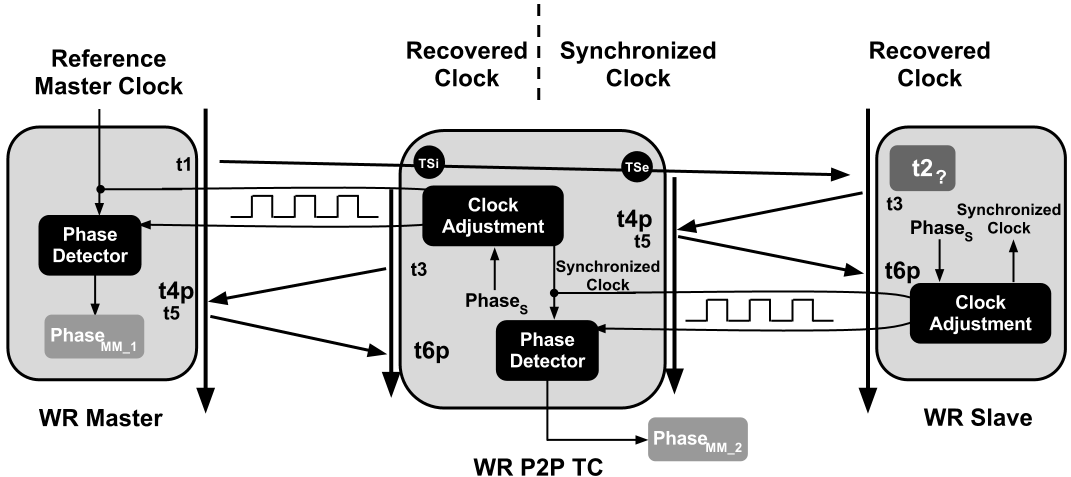
\includegraphics[scale=0.43]{fig/time_stamps_tc.png}
\caption{WR synchronization and P2P TC}
\label{fig:time_stamp}
\end{figure*}


\subsection{Time Stamping Accuracy}

As explained in Section~\ref{sec:wr}, the author resumes how WR accomplish
sub-nanoseconds synchronization and picoseconds jitter. It is based on the
characterization of the asymmetries of the link a priori, and a clock lookback
technique. By doing this WR is able to  enhance the timestamps on ingress ports. 

%\FloatBarrier
Figure~\ref{fig:time_stamp} shows that the Peer Delay timestamps between two 
adjacent nodes can be enhanced since the $phase_{MM\_1}$ and $phase_{S\_1}$ to
the reference master clock signal are known. But it is not the case for $t_{2}$, 
this timestamp can be only enhanced using $phase_{S\_2}$ since the reference clock 
signal used in this link, is a synchronized clock to the reference master clock
signal. The calculation of $offset_{ms}$ will be affected by the relative
enhancement. In the case of E2E TC all the timestamps on ingress port in the slave, are
not enhanced. Further understanding and investigation of enhancement of 
timestamps across TCs is needed.


\subsection{Correction Factor Stability and Maximum Update Rate}

Both, \textit{correction factor} (CF) and  \textit{update rate} (UR), are features greatly influenced
by the latency in the TC. As a result, synchronization could suffer
a degradation of performance. Long residence time in a TC is associated 
with an increase of traffic load handled by this TC. The authors of~\cite{biblio:tc_perf} 
present the parameter \textit{Correction Factor Error} (CFE). It expresses the difference of the latency measured by a 
test equipment and the updated CF. The authors test TCs from different vendors
under high multicast load and compare the CFE result. 
The outcome of the test clarifies that switches with hardware treatment of the Sync messages 
still maintain low the CFE value when the latency increases due to an increment
of traffic. WRS enjoys already hardware implementation 
of the timestamping unit, as well as hardware process forwarding of the messages.

The UR for a two-step clock, is defined as the time between the transmission of a Sync
message from the master till the reception of the Follow Up message by the slave. 
High latencies, 10-30\%~\cite{biblio:tc_perf} of the UR, can create 
instability in the slave. In addition, high latencies makes the TC unsuitable for applications
demanding high UR. WRS is designed to provide low latency for time critical
information (e.g control accelerator information) using Cut-Through forwarding
schema and QoS~\cite{biblio:vlan} in the output ports. 

\begin{figure}[!t]
\centering
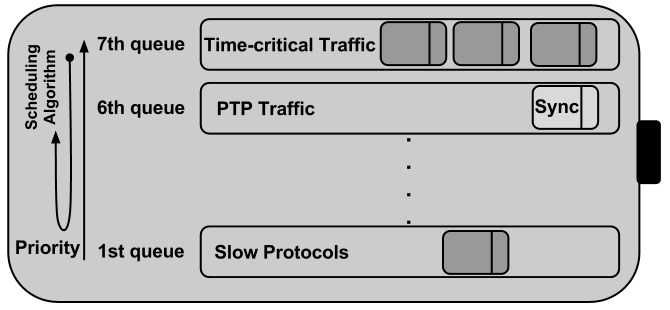
\includegraphics[scale=0.35]{fig/wr_port.png}
\caption{Queues in Output Port}
\label{fig:queue}
\end{figure}


Thus, PTP traffic can be queued in the second highest priority like Figure~\ref{fig:queue} 
shows. The queue scheduling algorithm is in charge to decide from which queue packets
are sent. The highest priority, 7th queue, is always emptied before the others,
and right after, the algorithm orders to check the PTP queue. If there is a  PTP message, it is sent
immediately. In this case, the delay in the switch would be affected only by
time-critical traffic and not by the rest of the traffic. Table~\ref{tab:delay}
presents an estimation of the delay between the Sync transmission and the Follow Up message reception
in a WR network made of five layer of switches. In this estimation, time-critical traffic is issued in burst of 
packets every 500 $\mu s$. The queue scheduling algorithm grantees that the maximum latency in the WRS for PTP traffic is 10 $ms$. The UR in this scenario could be around 20 Hz.

\begin{table}[!t]
\caption{Sync Transmission - Follow Up Reception Delay Estimation}
\centering
\begin{tabular}{l c }   
\hline
Number WRS & 5  \\
Time-critical Traffic burst period & 500 $\mu s$ \\
\hline
 \textbf{Delay}              &  \textbf{Max Value}     \\  \hline \hline
 Syn to Follow Up Tx            & 2 $ms$    \\ \hline
 White Rabbit Switch            &     10 $ms$      \\ \hline
\hline
 \textbf{Total}                          &  52 $ms$          \\
\hline
\end{tabular}
\label{tab:delay}
\end{table}

\subsection{Reconfiguration after Topologies Changes}

The use case of the timing system defines not only the requirements of accuracy
and precision, but also the stability and resilience of the synchronization in the event
of failures of TCs. The author doesn't find references of this features for timing system based on PTP in the
literature. Nevertheless, as the Table~\ref{tab:req} shows the new timing system for GSI and CERN  have a demanding requirement
regarding the synchronization accuracy. 

\begin{table}[!t]
\caption{GSI and CERN Timing System Requirements}
\centering
\begin{tabular}{l c c } 
\hline
    & \textbf{GSI} & \textbf{CERN} \\  \hline \hline
  Accuracy & 8 $ns$ & 1 $\mu s$  \\  \hline
  $d_{max}$ WR Master & 2 km & 10 km \\ \hline  
\end{tabular}
\label{tab:req}
\end{table}

Both timing systems achieve resilience against network failures using redundant
topologies. Lower layer protocols establish a spanning tree network and set ports connected to cyclic paths to block/passive
state to avoid loops. In this case only the P2P TC still issues the synchronization between the
ports in both directions. As a result both clocks have the link delay
information. This offers the possibility of having immediate availability of a
link after change in the topology. It means that the reconfiguration time 
doesn't depend on the TC anymore but on the  lower layer protocol. WRS has already 
proposals for implementing a transparent mechanism~\cite{biblio:wrswitch} for
recovering from single points of failure in a redundant network.
